\documentclass[12pt]{report}
\usepackage[margin=1in]{geometry}
\usepackage{hyperref}
\usepackage{graphicx}
\usepackage{amsmath}
\usepackage{enumitem}
\usepackage{float}

\title{Week 4 Report}
\author{Dhanush Balusa}
\date{June 11, 2025}

\begin{document}

\maketitle

\chapter*{Research}

\textbf{Error in TLE \& SGP4}
\begin{itemize}
  \item \textbf{Resource 1:} \url{https://conference.sdo.esoc.esa.int/proceedings/sdc6/paper/41/SDC6-paper41.pdf}
        \item TLEs are not suitable for precise orbit estimation because of innacuracies in modeling, timeliness, and inconsistency of the available orbital information.
        \item TLEs only accurate to about 2-3 days after the epoch. A week later, the error grows significantly.
        \begin{figure}[H]
          \centering
          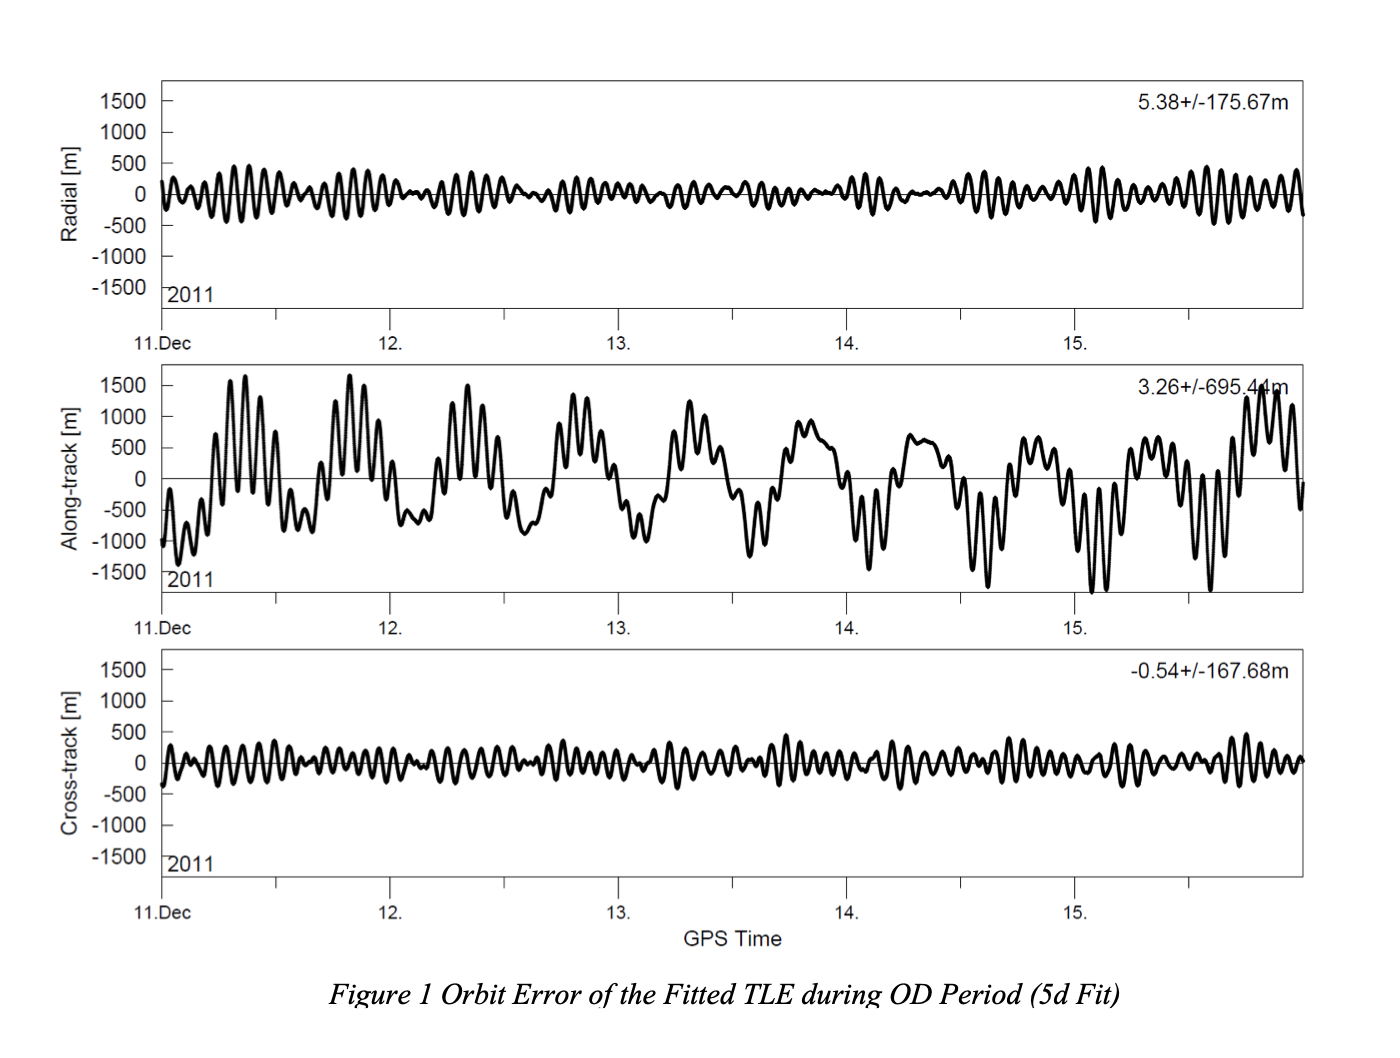
\includegraphics[width=0.8\textwidth]{figure_week_4_SGP4-error.png}
          \caption{Different types of error in SGP4 over a period of 5 days.}
          \label{fig:SPG4_error}
        \end{figure}

  \item \textbf{Resource 2:} \url{https://www.researchgate.net/profile/Eberhard-Gill-2/publication/224781886_Real-Time_Estimation_of_SGP4_Orbital_Elements_from_GPS_Navigation_Data/links/54ddb8d80cf28a3d93fa2e31/Real-Time-Estimation-of-SGP4-Orbital-Elements-from-GPS-Navigation-Data.pdf}
        \item Using SGP4, the initial position and speed will have a small error. These small errors at the start (called "at epoch") usually stay small, unless they affect the semi-major axis (SMA).
        \item If the SMA is off by a small amount (~10 meters), it slowly causes the satellite to get ahead or fall behind in its orbit (called along-track error). This error grows about 1 to 1.5 km per day.
        \item Good news? Using the filter (called RTSGP4), the SMA gets corrected quickly - within 1 day, the error becomes less than 10 meters.
        \begin{figure}[H]
          \centering
          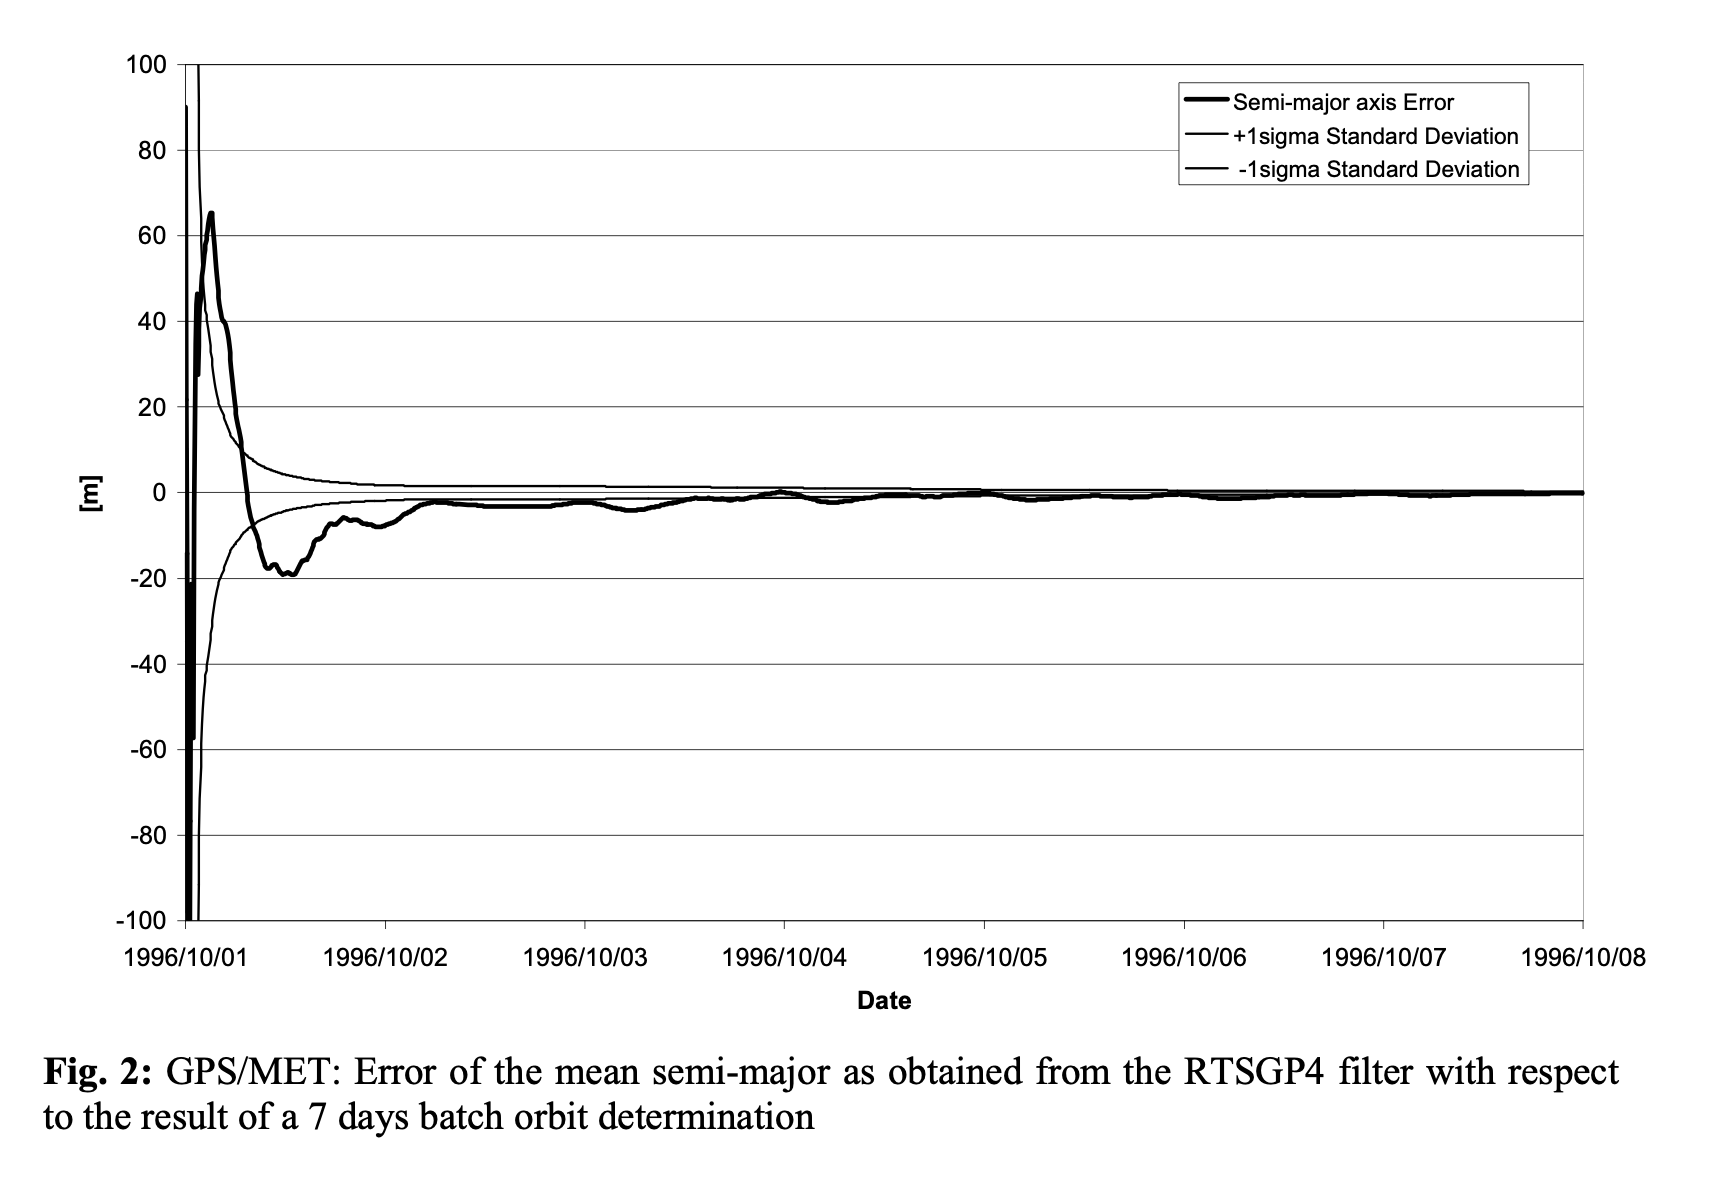
\includegraphics[width=0.8\textwidth]{figure_week_4_SGP4-RTSGP4.png}
          \label{fig:SPG4_error_RTSGP4}
        \end{figure}
        \item Summary: SGP4, when coupled with real-time mean-element estimation and drag-coefficient updating, can deliver sub-kilometre prediction accuracy over ~12–24 h—good enough to feed the ISS’s higher-precision conjunction assessment pipeline. Left unrefined, its along-track drift grows too large for reliable collision modeling.
\end{itemize}

\textbf{Other resources:}
\begin{itemize}
  \item \url{https://ntrs.nasa.gov/api/citations/20160005313/downloads/20160005313.pdf}
\end{itemize}

\textbf{Data Analysis from last week's collision event:}
\newline
\textbf{The key takeaways:}
The regular sinusoid makes sense because satellites in LEO orbit Earth every ~90 minutes, so the position appears to oscillate rapidly within 2 days. That would be around 32 orbits so the graph would have ~32 periods, which it does. I counted an there were 29 periods in the graph so that is close enough.
The sinusoid within the sinusoid is likely due to the error when using SGP4 to predict the position of the satellite. Although I didn't properly understand the error analysis for SPG4, it does seem like the error is periodic.

\chapter*{Previous Code}
My code from the previous week calculated the approach conditions between the collision of Iridium 33 and Cosmos 2251.

\begin{figure}[H]
    \centering
    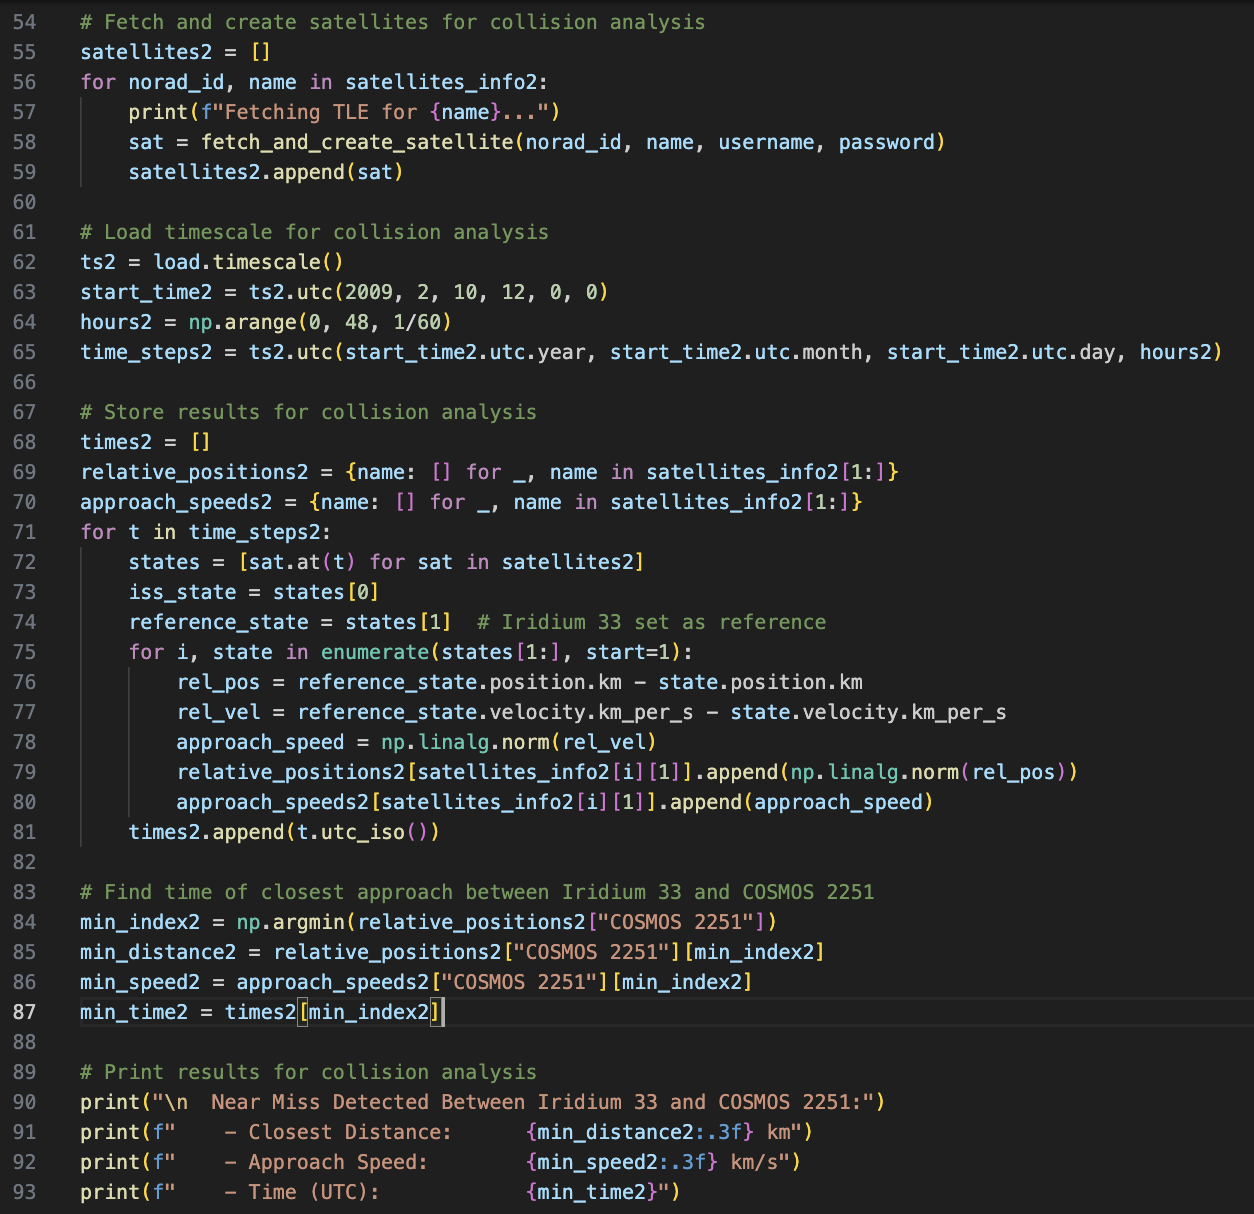
\includegraphics[width=0.8\textwidth]{figure_week_4_code.png}
    \caption{Code from week 4 calculating the approach conditions between the collision of Iridium 33 and Cosmos 2251}
    \label{fig:code}
\end{figure}

\chapter*{Code Changes}

Based on the feedback from last week’s team meeting, I decided to make the following changes:

\begin{enumerate}
  \item \textbf{My first change in the code was to check when I am pulling the data.}
  Here is the snippet of the code that I added to check the epoch of the satellites's TLEs I am pulling:
  \begin{verbatim}
  for sat in satellites2:
    print(f"{sat.name} Epoch: {sat.epoch.utc_iso()}")
  \end{verbatim}

  Here is the output of the code:
  \begin{verbatim}
    ISS (ZARYA), Epoch: 2009-02-10T21:26:33Z
    IRIDIUM 33, Epoch: 2009-02-10T18:16:11Z
    COSMOS 2251, Epoch: 2009-02-10T18:09:29Z
  \end{verbatim}

  Observation: The epoch of the TLEs I am pulling are from February 10, 2009 but they are at past 18 UTC.
  I wonder how my code was accurately able to calculate the collision was exactly at 16:56 UTC on February 10, 2009.
  It's good to know that I am able to pull historical TLEs from CelesTrak, but I wonder how I'm still able to calculate the collision time accurately.
  I'm not sure if I can find a TLE closser to the collision time than this so 2 hours of a difference is the best I can do, and plus the data looks accurate.

  \item \textbf{My second change in the code was to add the calculation of the approach angle.}

  \begin{figure}[H]
    \centering
    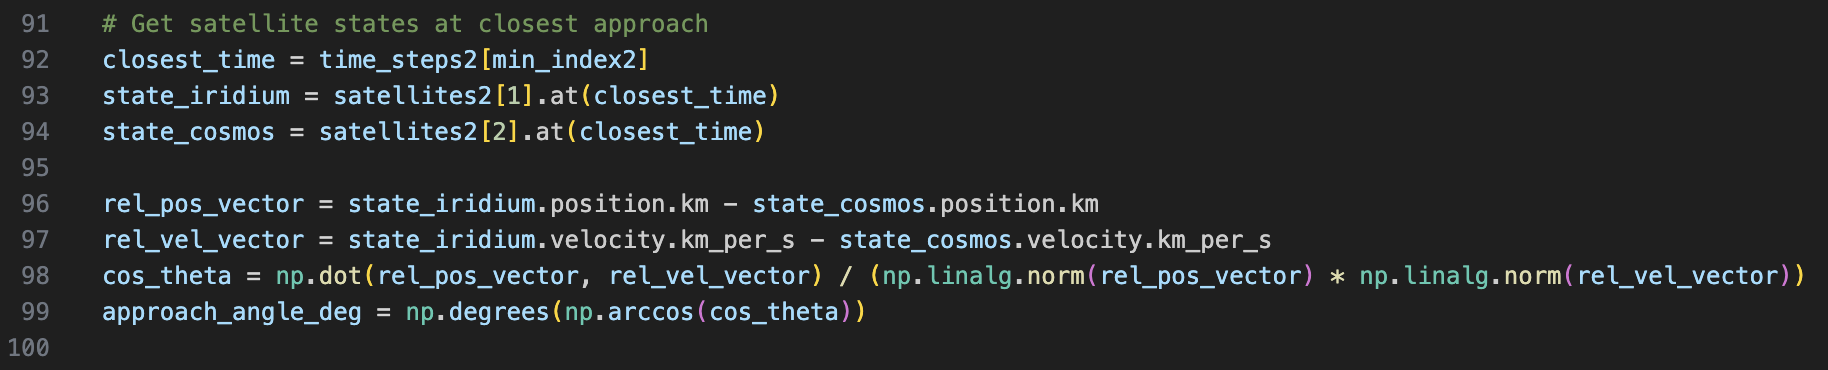
\includegraphics[width=0.8\textwidth]{figure_week_4_angle-code.png}
    \caption{Approach angle logic for Iridium 33 collision with Cosmos 2251.}
    \label{fig:iridium_collision_approach_angle}
  \end{figure}

  The code calculates the \textbf{approach angle} between two satellites by measuring the angle between their \textit{relative position vector} and the \textit{velocity vector} with respect to the first satellite (Iridium 33 in this case).
  \newline\newline
  This is computed using the dot product formula:
  \begin{equation}
  \theta = \arccos\left(\frac{\vec{r} \cdot \vec{v}}{|\vec{r}| |\vec{v}|}\right)
  \end{equation}

  where:
  \begin{itemize}
    \item $\vec{r}$ is the relative position vector between the two satellites (from Cosmos 2251 to Iridium 33),
    \item $\vec{v}$ is the relative velocity vector (how fast and in what direction Iridium 33 is moving relative to Cosmos 2251),
    \item $\theta$ is the angle between the two vectors.
  \end{itemize}

  The result is initially in radians and is then converted to degrees for easier interpretation.
  \newline\newline
  This approach angle provides insight into the geometry of the encounter:
  \begin{itemize}
    \item An angle near $0^\circ$ indicates a \textit{head-on approach}.
    \item An angle near $90^\circ$ suggests a \textit{tangential or glancing pass}.
    \item An angle near $180^\circ$ implies the satellites are moving in \textit{opposite directions}.
  \end{itemize}

  In this case, the code outputs an approach angle of \textbf{20.592°} for the Iridium 33 and Cosmos 2251 event.
  I have to understand how to interpret the angle correctly, by the looks of it from visual plots, the two satellites didn't really have a head-on collision, I would think the output would be closer to +$90^\circ$.
  \newline\newline
  I tried to use GMAT to visualize the collision but I was unable to get GMAT to work on my Mac and the school's virtual machine was not working either. I will try to get it working next week.
  For now, I have visual confirmation from NASA's resource about the collision.

  \begin{figure}[H]
    \centering
    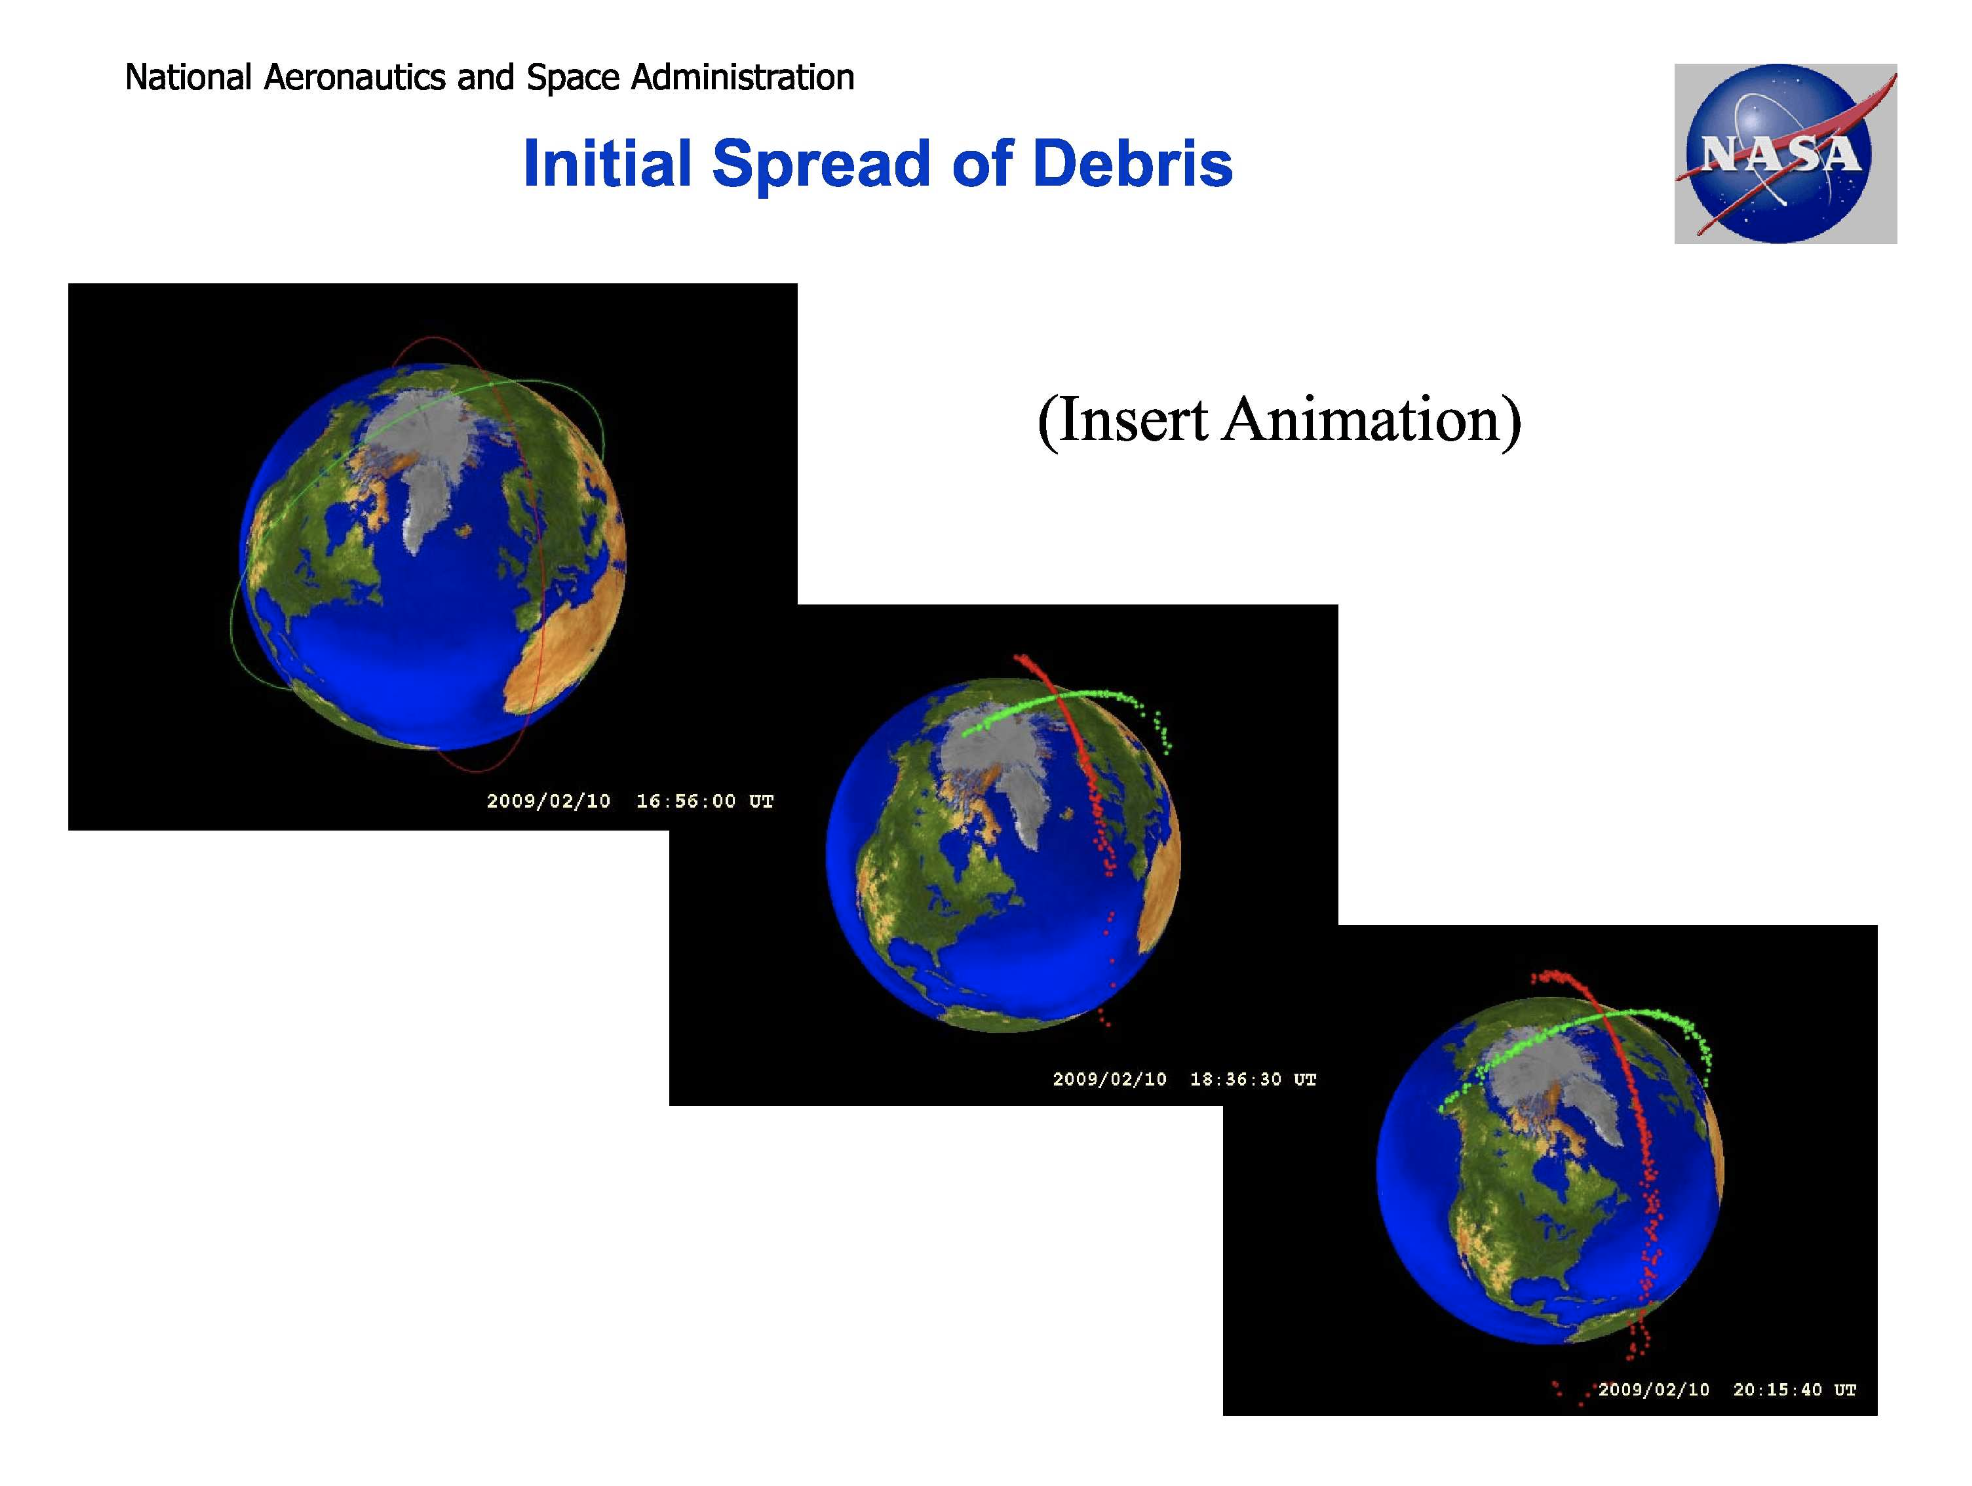
\includegraphics[width=0.8\textwidth]{figure_week_4_collision.png}
    \caption{Visualization of the Iridium 33 collision with Cosmos 2251.}
    \label{fig:collision_visualization}
  \end{figure}

  \begin{figure}[H]
    \centering
    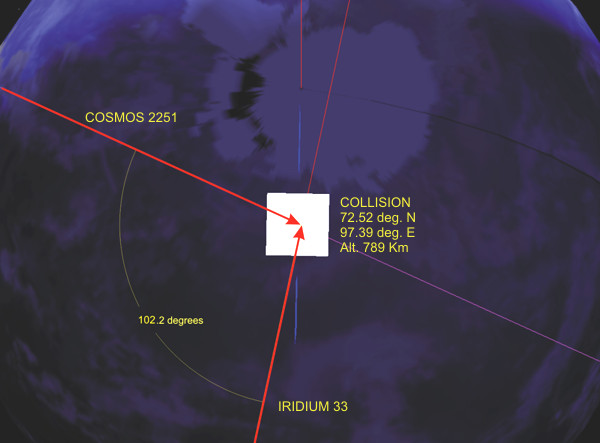
\includegraphics[width=0.8\textwidth]{figure_week_4_collision-wiki.png}
    \caption{Visualization of the collision on Wikipedia.}
    \label{fig:collision_visualization}
  \end{figure}

\end{enumerate}

\chapter*{Next Steps}
\begin{itemize}
  \item Further investigate the approach angle calculation and how to interpret it correctly.
  \item Try opening GMAT again to visualize the collision and the approach angle.
  \item Try other new senerios of collisions. Consider making my own senerios with TLEs that I can create.
  \item Monte Carlo simulation.
  \newline\newline\newline\textbf{Incomplete Goals from last week:}
  \item Loop through all the TLEs in the LEO category and calculate the approach conditions for each satellite if it is within a certain distance (e.g., 100 km) of the ISS.
  \item Make my code a usable function so Catherine can just call it. Input? \textrightarrow{} Output (angle and approach speed)
\end{itemize}

\end{document}